%! Author = zhenxiang
%! Date = 2023/3/27

\PassOptionsToPackage{quiet}{xeCJK}  % 抑制无意义的警告
% Preamble
\documentclass[11pt]{ctexart}


% Packages
\usepackage{amsmath,amssymb}
% graphicx
\usepackage{graphicx}
% 页面设置
\usepackage{geometry}
\geometry{left=2.5cm, right=2.5cm, top=2.5cm, bottom=2.5cm}
% codes
\usepackage{listings}
\usepackage{xcolor}
\usepackage{color}
\definecolor{mygreen}{rgb}{0,0.6,0}
\definecolor{mygray}{rgb}{0.5,0.5,0.5}
\definecolor{mymauve}{rgb}{0.58,0,0.82}
\lstset{ %
	backgroundcolor=\color{white},   % choose the background color; you must add \usepackage{color} or \usepackage{xcolor}
	basicstyle=\ttfamily,            % the size of the fonts that are used for the code
	breakatwhitespace=false,         % sets if automatic breaks should only happen at whitespace
	breaklines=true,                 % sets automatic line breaking
	captionpos=b,                    % sets the caption-position to bottom
	commentstyle=\ttfamily\color{mygreen},
	% comment style
	deletekeywords={},               % if you want to delete keywords from the given language
	escapeinside={},                 % if you want to add LaTeX within your code
	extendedchars=true,              % lets you use non-ASCII characters; for 8-bits encodings only, does not work with UTF-8
	frame=single,                    % adds a frame around the code
	keepspaces=true,                 % keeps spaces in text, useful for keeping indentation of code (possibly needs columns=flexible)
	keywordstyle=\color{blue},       % keyword style
	language=bash,                    % the language of the code
	morekeywords={},                 % if you want to add more keywords to the set
	numbers=left,                    % where to put the line-numbers; possible values are (none, left, right)
	numbersep=5pt,                   % how far the line-numbers are from the code
	numberstyle=\tiny\color{mygray}, % the style that is used for the line-numbers
	rulecolor=\color{black},         % if not set, the frame-color may be changed on line-breaks within not-black text (e.g. comments (green here))
	showspaces=false,                % show spaces everywhere adding particular underscores; it overrides 'showstringspaces'
	showstringspaces=false,          % underline spaces within strings only
	showtabs=false,                  % show tabs within strings adding particular underscores
	stepnumber=1,                    % the step between two line-numbers. If it's 1, each line will be numbered
	stringstyle=\color{mymauve},     % string literal style
	tabsize=2,                       % sets default tabsize to 2 spaces
	title=\lstname                   % show the filename of files included with \lstinputlisting; also try caption instead of title
}
%url
\usepackage{hyperref}
% ref
\usepackage{gbt7714}
\bibliographystyle{gbt7714-numerical}
%table
\usepackage{booktabs, tabularx, multirow}
% 字体
\usepackage{fontspec}
\usepackage{xeCJK}

\newcommand{\xbsong}{\CJKfamily{zhxbs}}
\newcommand{\dbsong}{\CJKfamily{zhdbs}}

\newcommand{\dahei}{\CJKfamily{zhdh}}
% 隶书
\setCJKfamilyfont{ls}{LiSu}                                                                                                                         
\newcommand{\lishu}{\CJKfamily{ls}} 
% 自定义命令
\newcommand{\EE}{\mathbb{E}}
\begin{document}
\tableofcontents
	
\section{You will get}

\begin{itemize}
	\item 环境配置、编辑器使用
	\item 简单操作
	\item 套用模板
	\item  遇到问题怎么解决
\end{itemize}

\newpage

\section{Install}

\subsection{安装介绍}



安装步骤,参考\href{https://github.com/OsbertWang/install-latex-guide-zh-cn/releases}{guide手册}

\href{https://www.tug.org/texlive/doc/texlive-zh-cn/texlive-zh-cn.pdf}{guide手册2}

从\href{https://mirrors.tuna.tsinghua.edu.cn/CTAN/systems/texlive/Images/}{清华下载镜像源 texlive2023.iso}

\begin{figure}[ht]
	\centering
	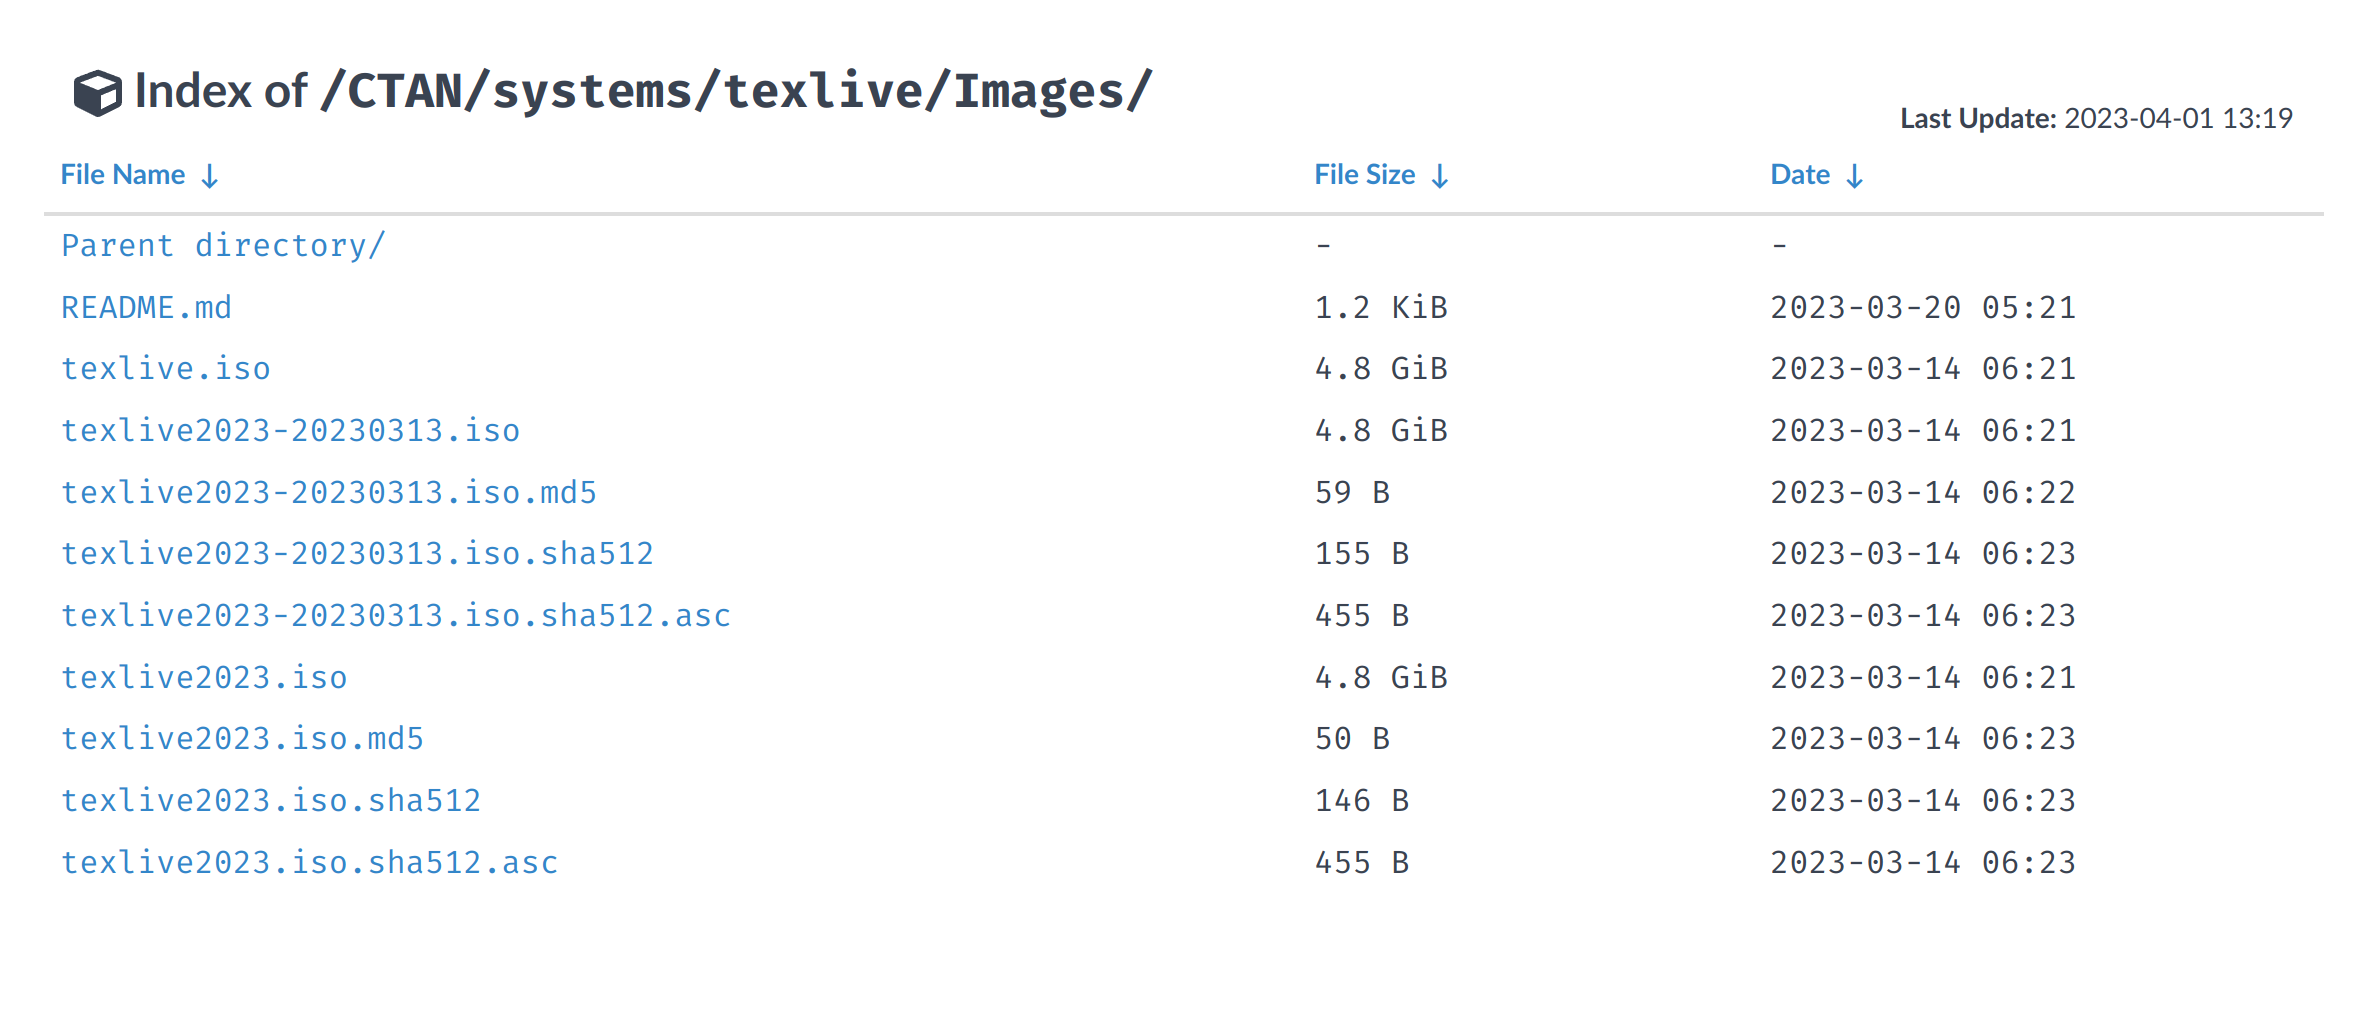
\includegraphics[width=1.0\textwidth]{images/texlive2023Images.png}
	\caption{镜像源~ 选择texlive2023.iso}
	\label{fig:2023image}
\end{figure}

安装过程

\begin{figure}[ht]
	\centering
	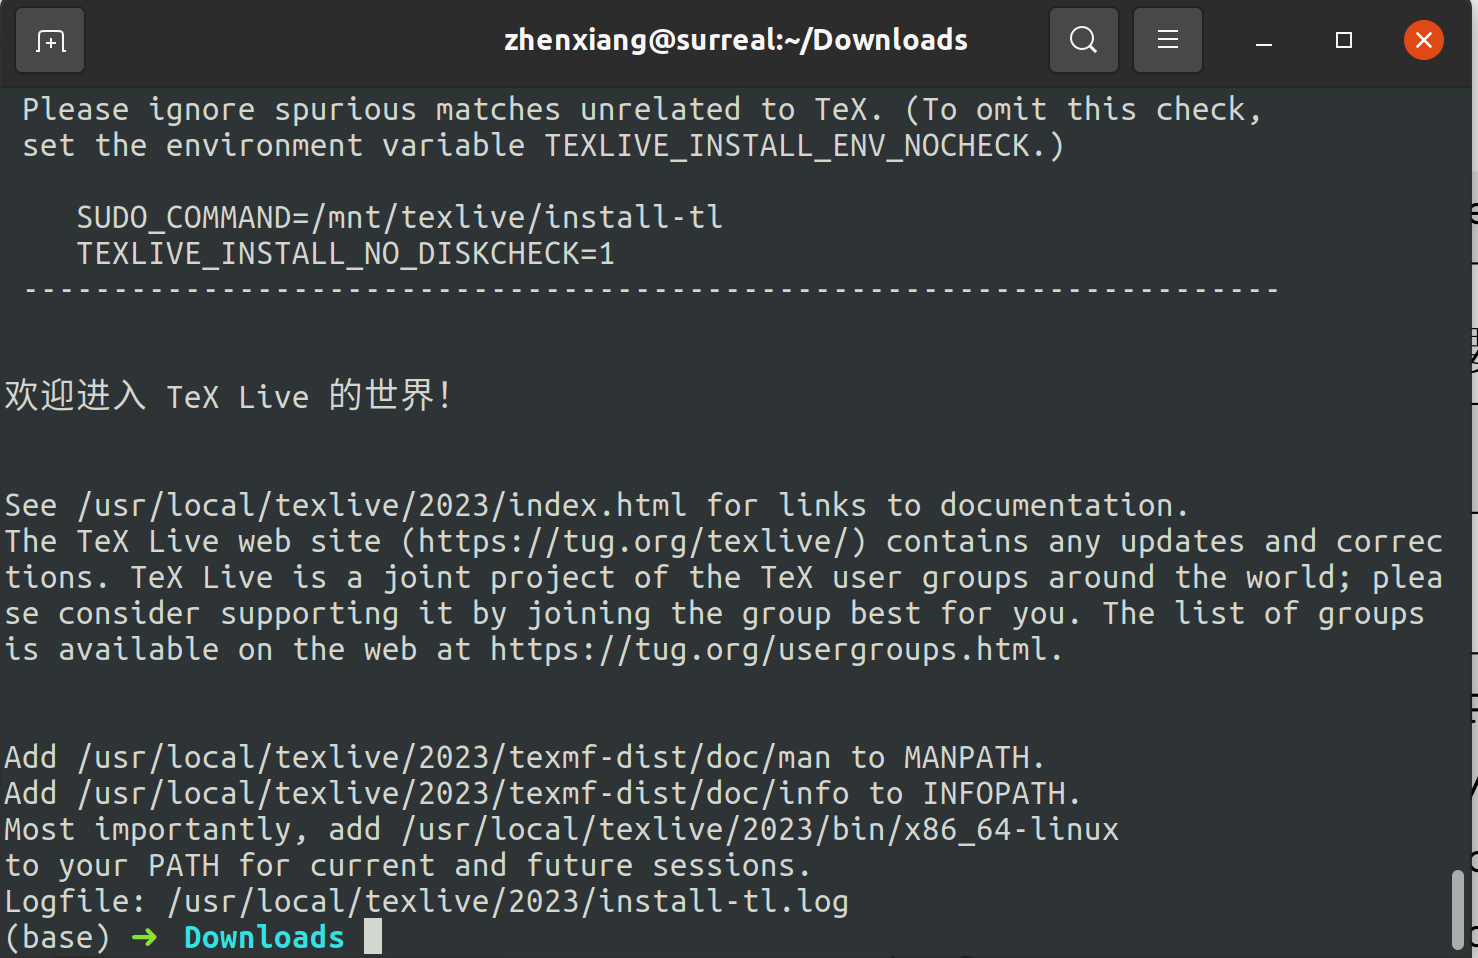
\includegraphics[width=0.4\textwidth]{images/installing_1.png}
	\qquad
	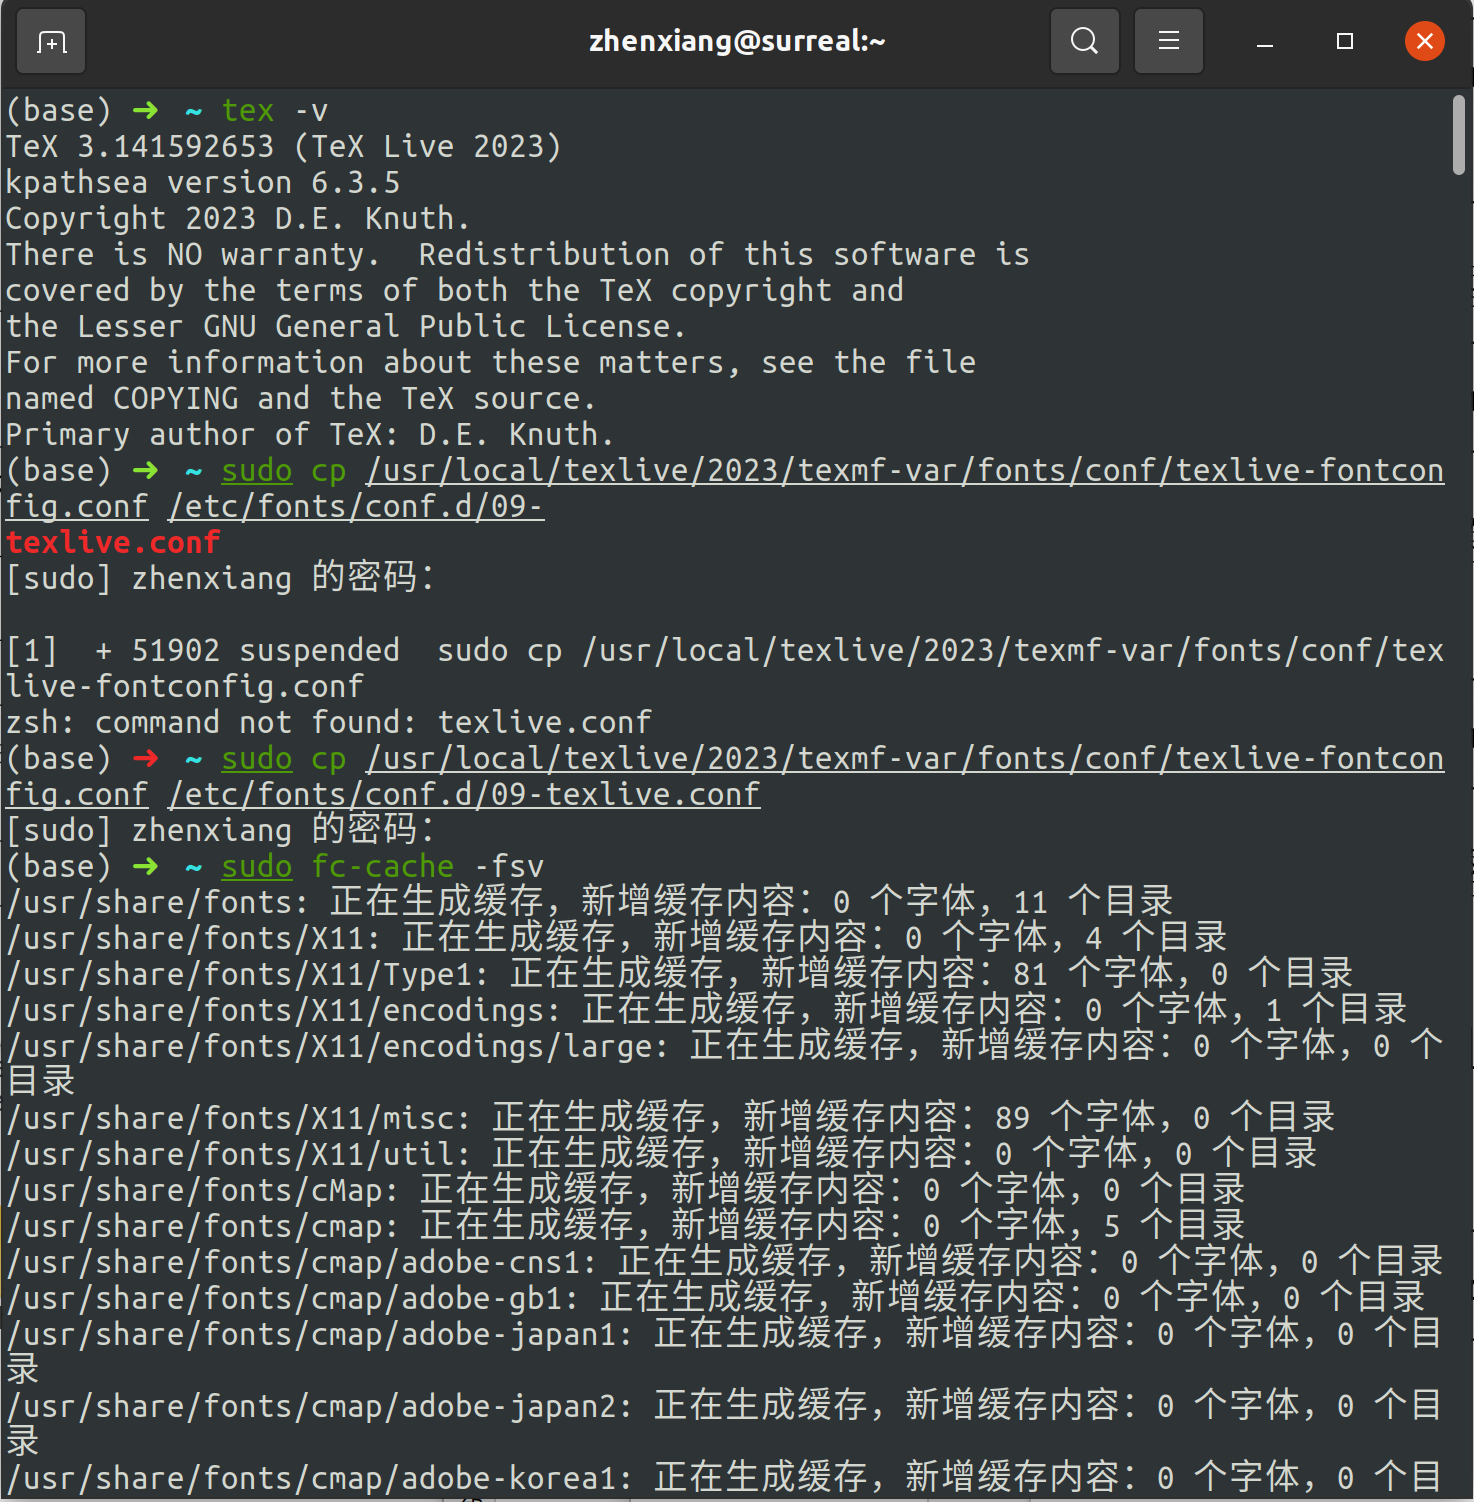
\includegraphics[width=0.4\textwidth]{images/installing_2.png}
	\caption{安装过程}
	\label{fig:install}
\end{figure}



\newpage

\begin{figure}[ht]
	\centering
	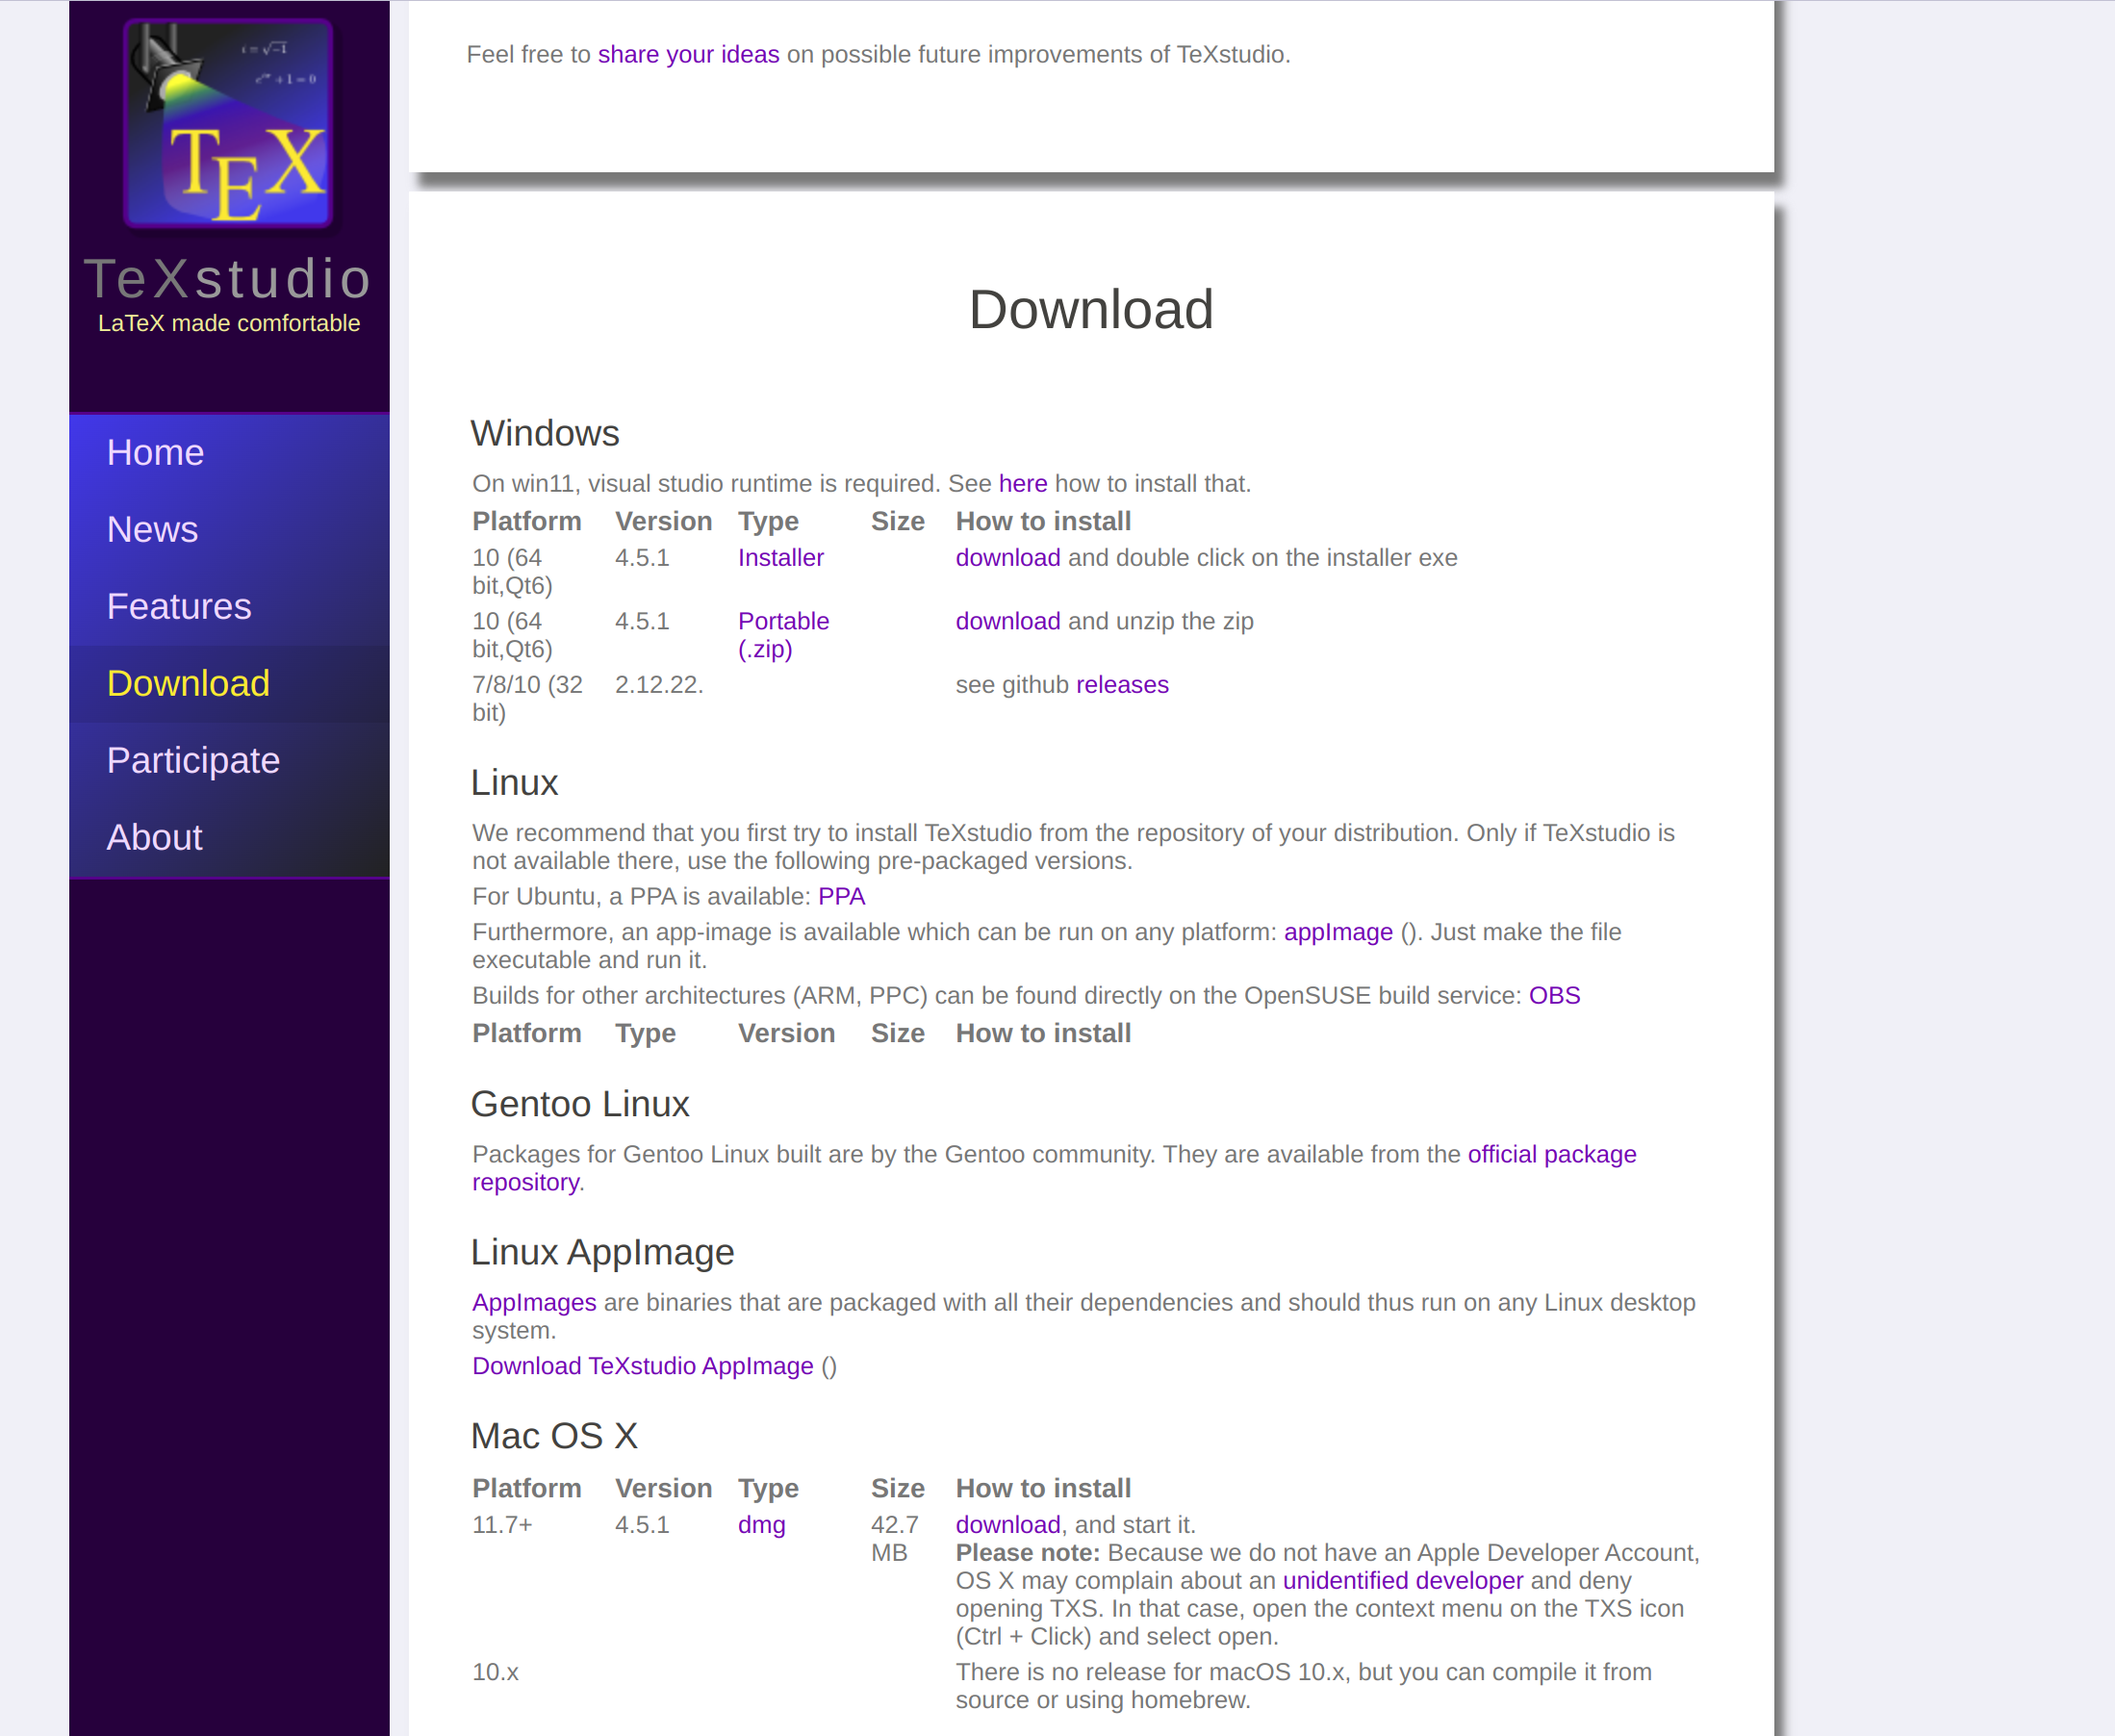
\includegraphics[width=0.5\textwidth]{images/texstudio.png}
	\caption{下载你的平台版本}
	\label{fig:texstudio}
\end{figure}

编辑器下载\href{https://www.texstudio.org/}{texstudio}



ubuntu下安装texstudio

\begin{lstlisting}
	sudo add-apt-repository ppa:sunderme/texstudio
	sudo apt update
	sudo apt install texstudio
\end{lstlisting}

以及其他编辑器 如texmaker 、jetbrains ( pycharm、clion ) 装插件、配置vscode


配置texlive2023环境变量

\begin{lstlisting}
	vi ~/.bashrc
	export PATH=/usr/local/texlive/2023/bin/x86_64-linux:$PATH
	export MANPATH=/usr/local/texlive/2023/texmf-dist/doc/man:$MANPATH
	export INFOPATH=/usr/local/texlive/2023/texmf-dist/doc/info:$INFOPATH
\end{lstlisting}




\newpage

\section{use}

\subsection{local}

\subsubsection{ 插入代码}

\begin{lstlisting}
	#include <llvm/Passes/PassBuilder.h>
	#include <llvm/Passes/PassPlugin.h>
	#include <llvm/Support/raw_ostream.h>
	
	using namespace llvm;
	
	namespace {
		
		class FunctionInfoPass final : public PassInfoMixin<FunctionInfoPass> {
			public:
			PreservedAnalyses run([[maybe_unused]] Module &M, ModuleAnalysisManager &) {
				outs() << "CSCD70 Function Information Pass"
				<< "\n";
				/// @todo(CSCD70) Please complete this method.
				for (auto &F : M.functions()) {
					outs() << "Function Name: " << F.getName() << "\n";
					outs() << "Number of Arguments: " << F.arg_size() << "\n";
					// Count direct call sites.
					int numDirectCalls = 0;
					for (User *U : F.users()) {
						if (auto *CI = dyn_cast<CallInst>(U)) {
							if (CI->getCalledFunction() == &F) {
								++numDirectCalls;
							}
						}
					}
					outs() << "Number of Calls: " << numDirectCalls << "\n";
					
					int numBasicBlocks = 0, numInstructions = 0;
					for (BasicBlock &BB : F) {
						++numBasicBlocks;
						for (Instruction &I : BB) {
							++numInstructions;
						}
					}
					outs() << "Number OF BBs: " << numBasicBlocks << "\n";
					outs() << "Number of Instructions: " << numInstructions << "\n";
				}
				//M.print(outs(), nullptr);
				return PreservedAnalyses::all();
			}
		}; // class FunctionInfoPass
		
	} // anonymous namespace
\end{lstlisting}


\subsubsection{插入公式}

\[
\mathbf{P}=
\begin{bmatrix}
	P(s_1|s_1) & P(s_2|s_1) & \ldots & P(s_N|s_1)\\
	P(s_1|s_2) & P(s_2|s_2) & \ldots & P(s_N|s_2)\\
	\vdots & \vdots & \ddots & \vdots\\
	P(s_1|s_N) & P(s_2|s_N) & \ldots & P(s_N|s_N)\\
\end{bmatrix}
\]




\begin{align*}
	V(s) & = \mathbb{E}[G_t|s_t=s] \\
	& = \mathbb{E}[\gamma r_{t+1} + \gamma^{2} r_{t+2} + \ldots + 		\gamma^{H-1} r_{t+H-1}|s_t=s]\\
	& = \mathbb{E}[r_{t+1}|s_t = s] + \gamma\mathbb{E}[r_{t+2}+\gamma r_{t+3}+\gamma^2 r_{t+4}+ \ldots | s_t = s]\\
	& = R(s) + \gamma\mathbb{E}[G_{t+1}|s_t = s] ~~~ &*\\
	& = R(s) + \gamma\mathbb{E}[V(s_{t+1})|s_t = s]  ~~~ &*\\
	& = \underbrace{R(s)}_\text{Immediate reward} + \underbrace{ \gamma\sum_{s' \in S}p(s' | s)V(s')}_\text{Discounted sum of future rewards}
\end{align*}

\newpage
\subsubsection{图片}

\begin{figure}[h]
	\centering
	
\includegraphics[width=0.5\textwidth]{images/LLVM.png}
	\caption{LLVM ~ LOGO}
	\label{fig:logo}
\end{figure}


 
 \subsubsection{表格}
 
 \begin{table}[h]
 	\centering
 	\caption{Expected \texttt{FunctionInfo} Output for \texttt{Loop.c}}
 	\begin{tabular}{*{5}{c}}
 		\toprule
 		Name & \# Args & \# Calls & \# Blocks & \# Insts \\
 		\midrule
 		\texttt{g\_incr} & 1 & 0 & 1 &  4 \\
 		\texttt{loop}    & 3 & 0 & 3 & 10 \\
 		\bottomrule
 	\end{tabular}
 	\label{functioninfo-loop-mb}
 \end{table}
 
 \subsubsection{字体设置}
 
 {\heiti\zihao{2} 黑体\qquad 追逐影子的人,自己就是影子。}
 
 {\songti\zihao{-2} 宋体\qquad 追逐影子的人,自己就是影子。}
 
    {\heiti\zihao{-4} 黑体\qquad 追逐影子的人,自己就是影子。}
 
 {\fangsong\zihao{-4} 仿宋\qquad 追逐影子的人,自己就是影子。}
 
 {\lishu\zihao{-4} 隶书\qquad 追逐影子的人,自己就是影子。}
 
  {\songti\zihao{-4} 宋体\qquad 追逐影子的人,自己就是影子。}
  
   {\kaishu\zihao{-4} 楷书\qquad 追逐影子的人,自己就是影子。}
   
   
   \begin{figure}[ht]
   	\centering
   	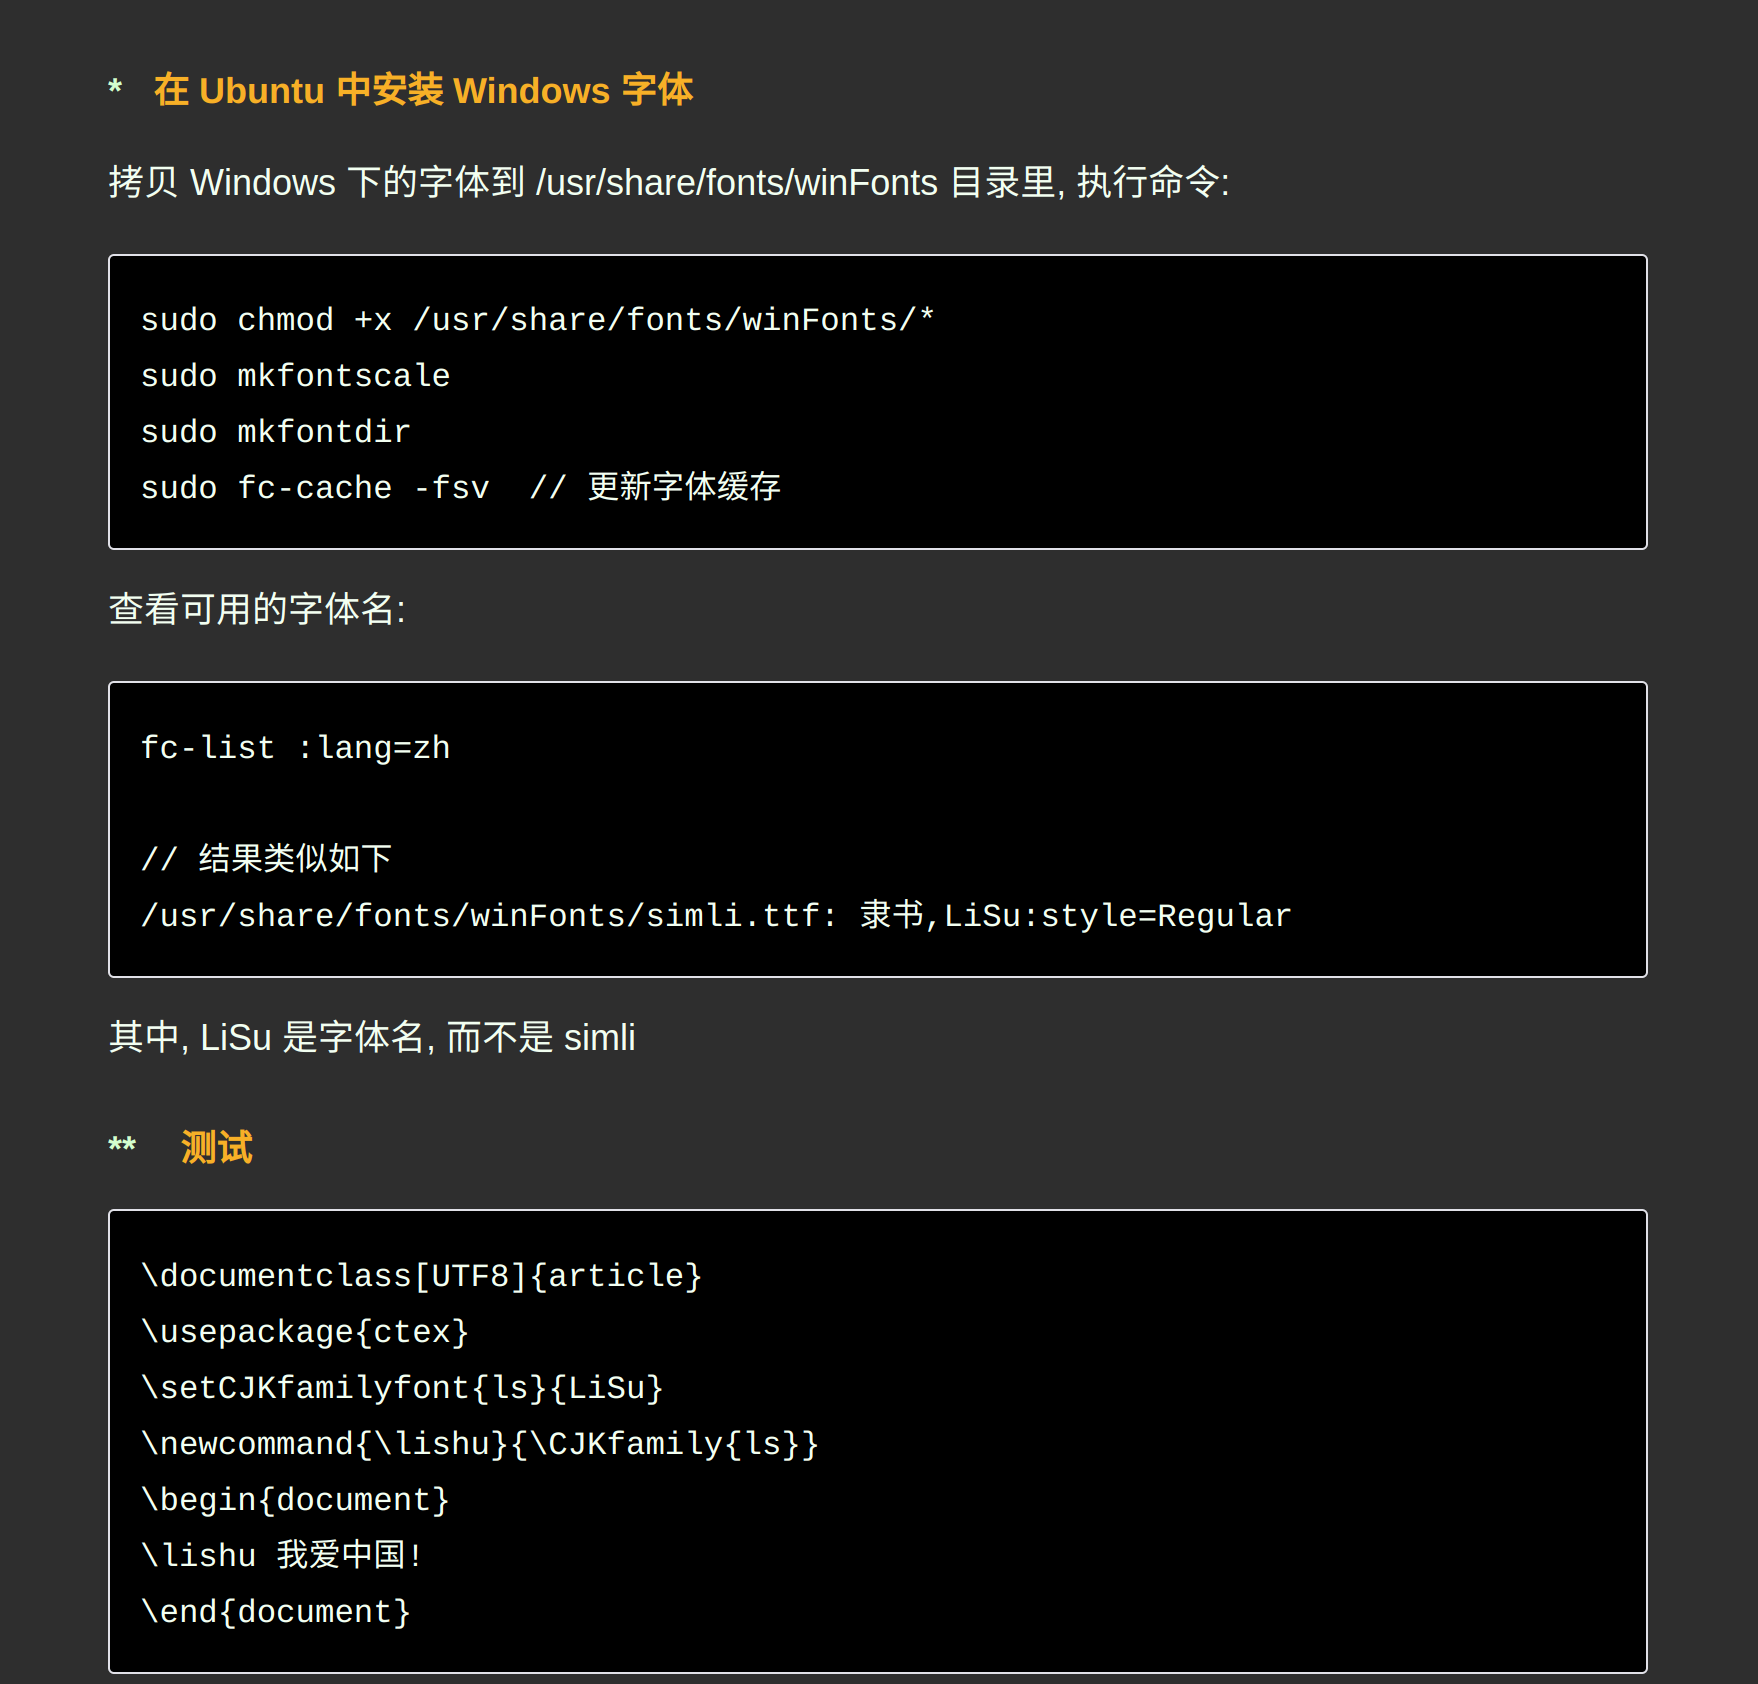
\includegraphics[width=0.5\textwidth]{images/font.png}
   	\caption{安装win平台字体}
   	\label{fig:setfont}
   \end{figure}
 \subsubsection{页面设置}
 \begin{lstlisting}
 	% 页面设置
 	\usepackage{geometry}
 	\geometry{left=2.5cm, right=2.5cm, top=2.5cm, bottom=2.5cm}
 \end{lstlisting}
 
 \subsubsection{目录}
 
 \begin{lstlisting}
 	\tableofcontents
 \end{lstlisting}
 
 \subsubsection{文件结构}
 
 \begin{itemize}
 	\item .sty 宏包文件。宏包的名称与文件名一致。
 	\item .cls 文档类文件。文档类名称与文件名一致。
 	\item .bib B IB TEX 参考文献数据库文件。
 	\item .log 排版引擎生成的日志文件,供排查错误使用。
 	\item .aux L A TEX 生成的主辅助文件,记录交叉引用、目录、参考文献的引用等。
 \end{itemize}
 

 
 \subsubsection{插入链接}
 
  在线的编辑器 \href{www.overleaf.com}{国际overleaf}
 
 \subsubsection{自定义命令}
 
 \begin{lstlisting}[language=tex]
 	\newcommand{\EE}{\mathbb{E}}
 \end{lstlisting}

\begin{equation}
	\mathbb{E}
\end{equation}

\begin{equation}
	\EE
\end{equation}
 
 \subsubsection{引用文献}
 
 \href{https://www.jabref.org/}{下载jabref}
 
 \begin{figure}[h]
 	\centering
 	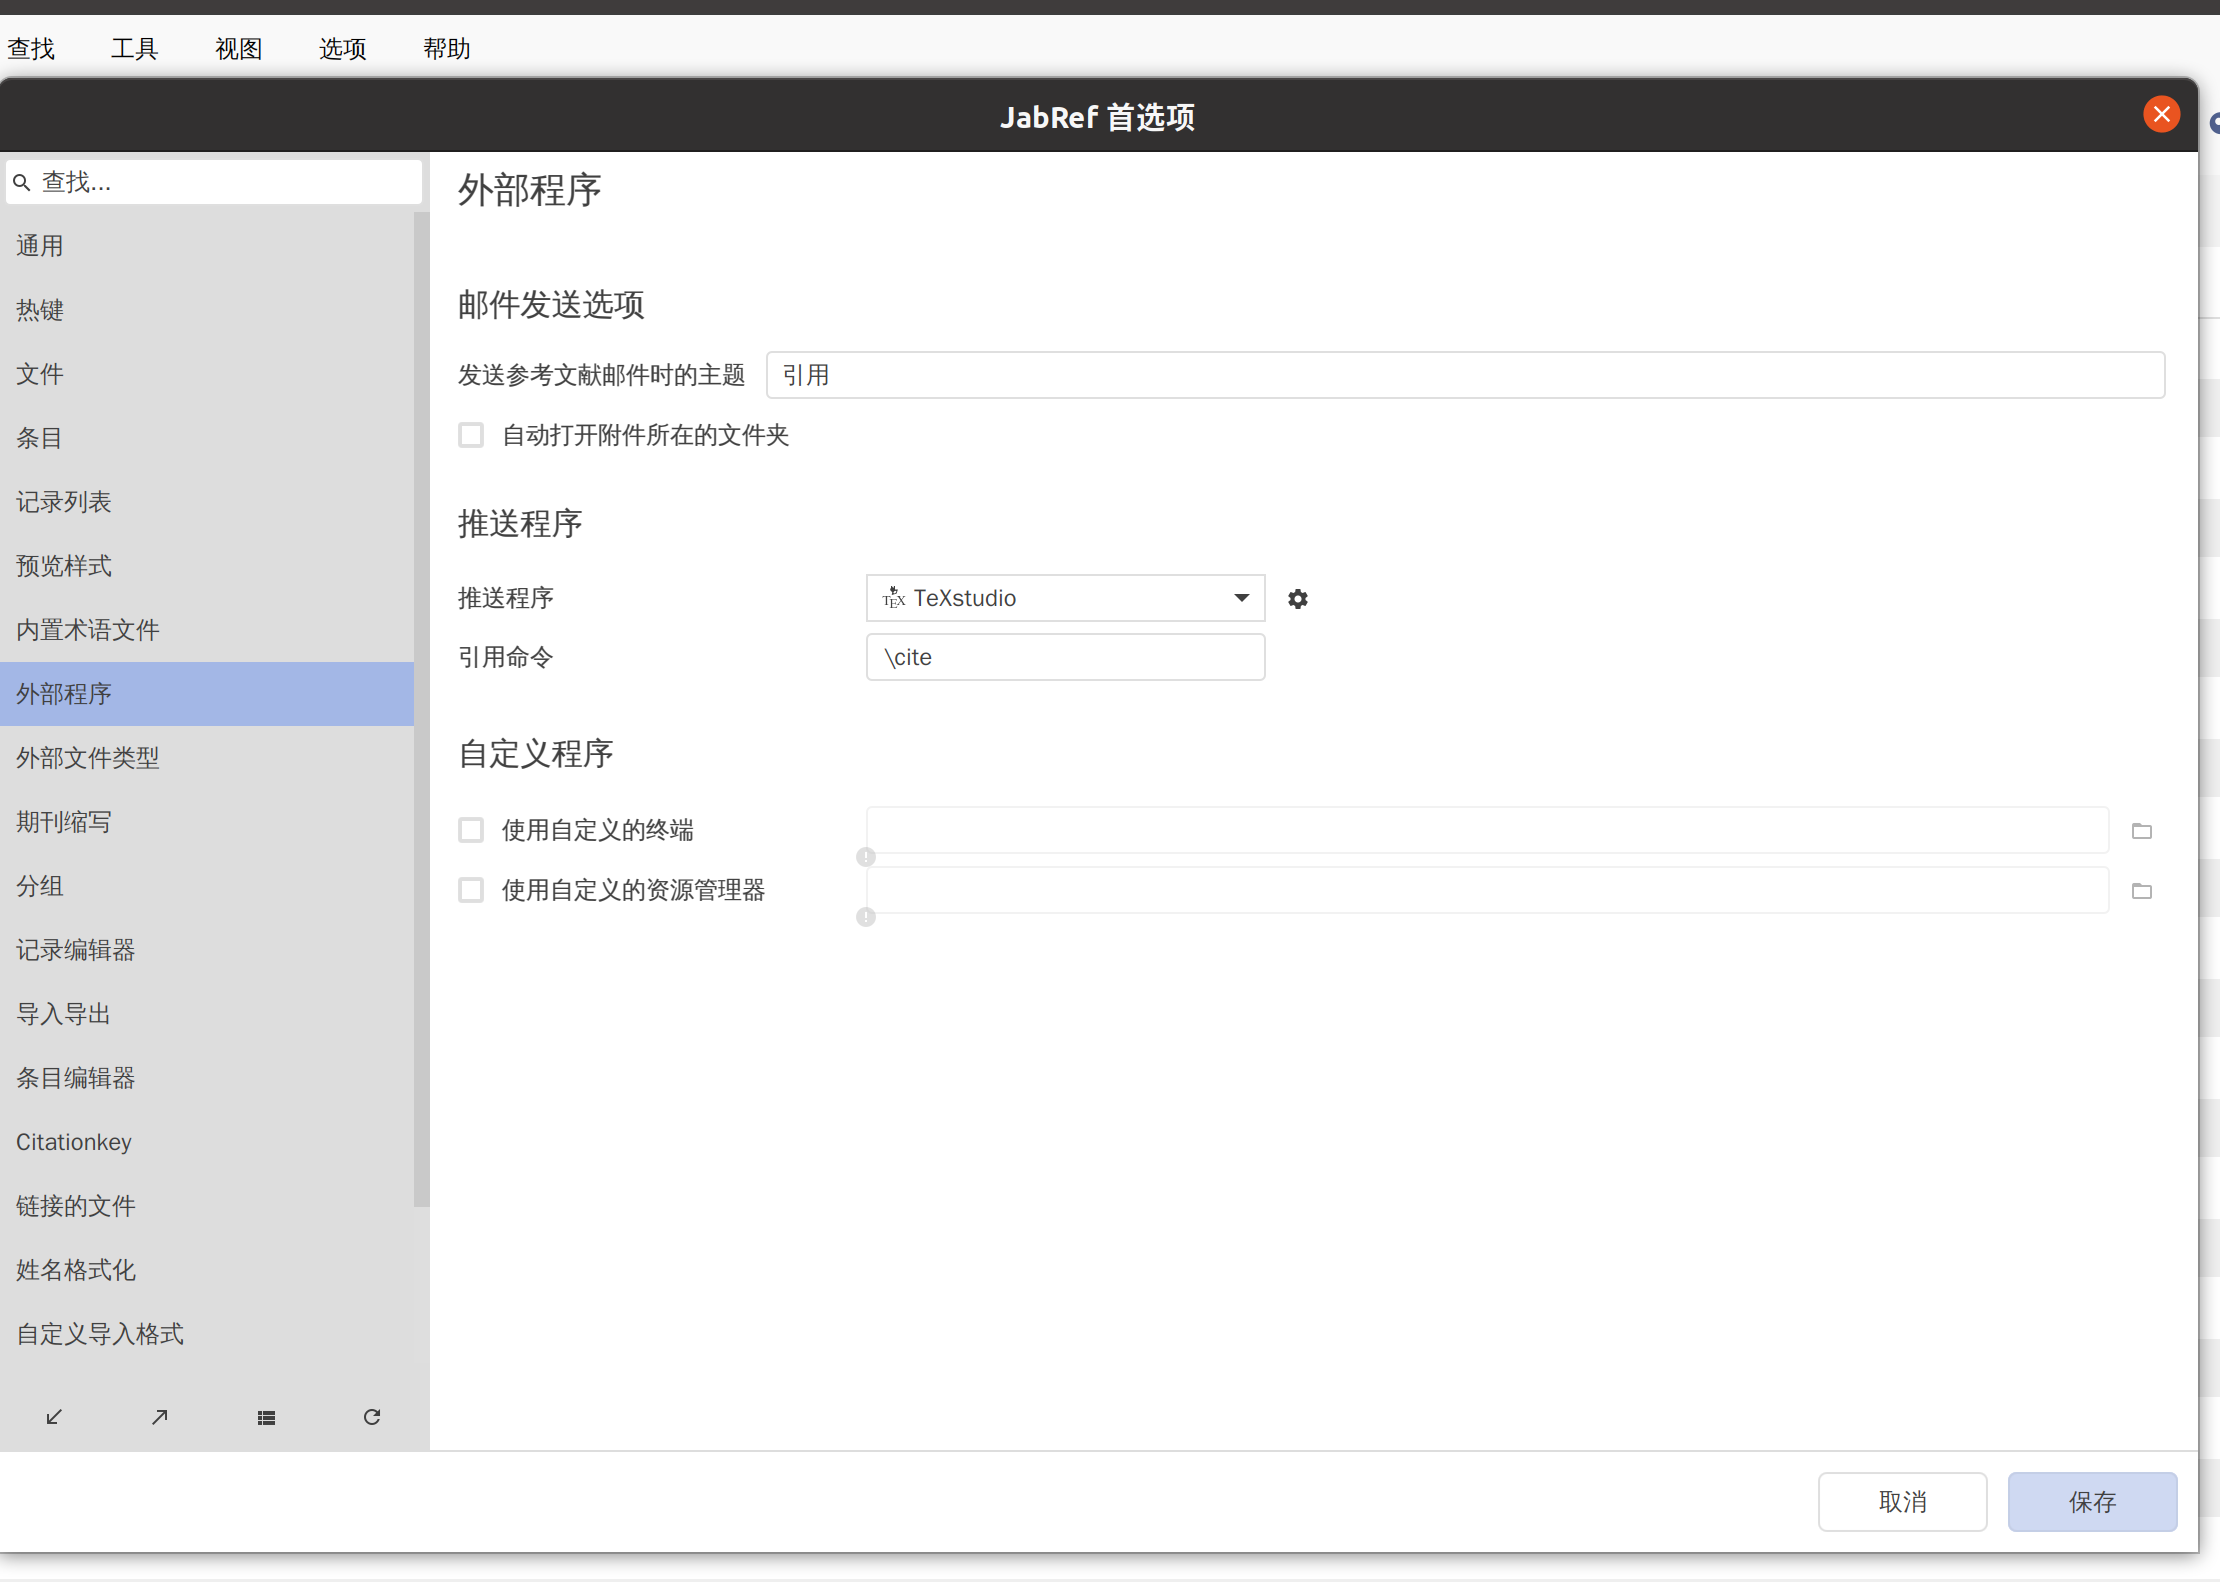
\includegraphics[width=0.5\textwidth]{images/jabref_set.png}
 	\caption{jabref设置}
 	
 \end{figure}
 
 \begin{lstlisting}
 	% ref
 	\usepackage{gbt7714}
 	\bibliographystyle{gbt7714-numerical}
 \end{lstlisting}
 
 Deep learning\cite{lecun2015deep}
 
 Causal confusion in imitation learning\cite{de2019causal}
 
 behavioral cloning\cite{wen2020fighting}
 
 
 \subsection{online}
 
 在线的编辑器 \href{www.overleaf.com}{国际overleaf}
 
 \href{cn.overleaf.com}{国内版本overleaf}
 
 国产的\href{www.texpage.com}{texpage}
 
 
 \subsection{for me personally}
 
 pycharm latex模板配置, pycharm实现git简单操作push到自己私有仓库,Texstudio编写tex文件
 
 \section{template}

使用模板, 以 imcl为例

\href{https://arxiv.org/}{arxiv}上下载latex版本文章
\section{solve problem}

 chatgpt,查阅文档  texdoc name





\section{reference}

https://github.com/CTeX-org/lshort-zh-cn/releases

https://github.com/xinychen/latex-cookbook

https://github.com/luong-komorebi/Begin-Latex-in-minutes

https://github.com/dspinellis/latex-advice

https://tug.org/

https://ctan.org/

https://texdoc.org/index.html

https://ctex.org/

https://tex.stackexchange.com/

https://www.mathcha.io/

https://www.latexlive.com/home\#\#


\bibliography{bib/ref_learn.bib}


\end{document}